
\subsection{Validation} Validation of models is important to ascertain that the results output are accurate. However, it should be noted that these long-term simulations are not predictions of the future, rather possible outcomes based upon certain assumptions. Therefore, the results from ElecSIM should be analysed by taking into account the underlying assumptions of the model, and comparing inputs to outcomes, as well as looking at the general trends that emerge.

Jager posits that a certain outcome or development path, captured by empirical data, might have developed in a completely different direction due to chance \cite{Jager2006a}. However, through observation, the processes that emerge from a model should be realistic and in keeping with expected behaviour \cite{Jager2006}.

We begin by comparing the price duration curve in the year 2018. Figure \ref{fig:price_duration_curve} shows the N2EX Day Ahead Auction Prices of the UK \cite{nordpool_2019}, the stochastic simulated electricity prices, and the non-stochastic electricity price throughout the year 2018. The N2EX Day Ahead Market is a day ahead market run by Nord Pool AS. Nord Pool AS runs the largest market for electrical energy in Europe, measured in volume traded and in market share \cite{nordpool_2019}.

The variance of the simulated stochastic runs were achieved by calculating the runs 40 times. Outliers were removed as on a small number of occasions large jumps in prices at peak demand occurred which deviated significantly from the mean. We did this, as although this does occur in real life, it occurs at a smaller fraction of the time than 5\% of the year (modelled load duration curve), therefore the results would be unreasonably skewed for the highest demand segment. However, we would expect these high prices to occur both in real life and in the model with a higher resolution price duration curve.

Figure \ref{fig:price_duration_curve} demonstrates very little variance in the non-stochastic case. This is because the majority of plants that set the spot price are combined cycle gas turbines (CCGTs). These CCGTs had little variance between one another as they were calibrated using the same data. By adding stochasticity of fuel prices and operation and maintenance prices, a curve that more closely resembles the actual data occurs. The stochastic curve, however, does not perfectly fit the real data, which may be due to higher variance in fuel prices and historical differences in operation and maintenance costs between power plants. One method of improving this would be fitting the data to the curve.

Table \ref{table:validation_metrics} shows performance metrics of the stochastic and non-stochastic runs versus the actual price duration curve . It can be seen that stochastic implementation (ElecSIM), improves the mean absolute error (MAE) by $52.5\%$.

%\addtolength{\textfloatsep}{-0.05in}
\begin{figure}
	\begin{center}
		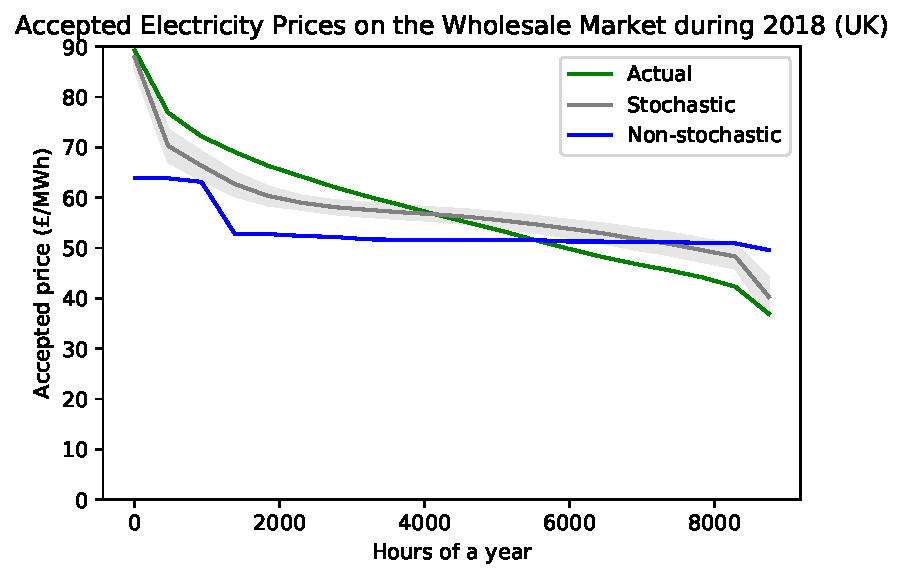
\includegraphics[width=0.5\textwidth]{figures/load_price_duration_curve_comparison.pdf}
		\caption{Price duration curve which compares real electricity prices to those paid in ElecSIM with and without stochasticity.}
		\label{fig:price_duration_curve}
	\end{center}
\end{figure}


\begin{table}
	\centering
	\csvautobooktabular{tables/validation/initialisation_run_validation.csv}
	\caption{Validation performance metrics.}
	\label{table:validation_metrics}
\end{table}
\addtolength{\textfloatsep}{-0.05in}

Therefore, the adding of stochasticity to fuel prices and variable operation \& maintenance improves on previous attempts of a yearly step model.

By observing the processes that emerge from the long-term scenarios, we can see that carbon price and investment in renewable generation are positively correlated, and is what one would expect.

We found that the net present value (NPV) calculations are realistic, with onshore wind and Combined Cycle Gas Turbines (CCGT) the technologies that are most invested in. It is true, within the United Kingdom, that Onshore wind and CCGT power generators are the most cost effective, and heavy government subsidies are required for other generation types such as nuclear and coal. 



\subsection{Performance}

 We used Microsoft Azure Public Cloud. Utilising two virtual machines of 64 vCPU's each (D64 v3), which are built using Intel Broadwell E5-2673 v4 2.3GHz processors, and the Intel Haswell 2.4 GHz E5-2673 v3. They have a combined total of 256GB of memory and use a Linux operating system. This enabled us to rapidly prototype different demand and carbon price scenarios, and run the simulation multiple different times to attain a variance in results.

The total disk size of ElecSIM is 380MB. The amount taken up by data and reports is 175MB, whilst the source code takes up 19.6MB. The memory used for a single run has a mean of 2GB.


\begin{figure}
	\centering
	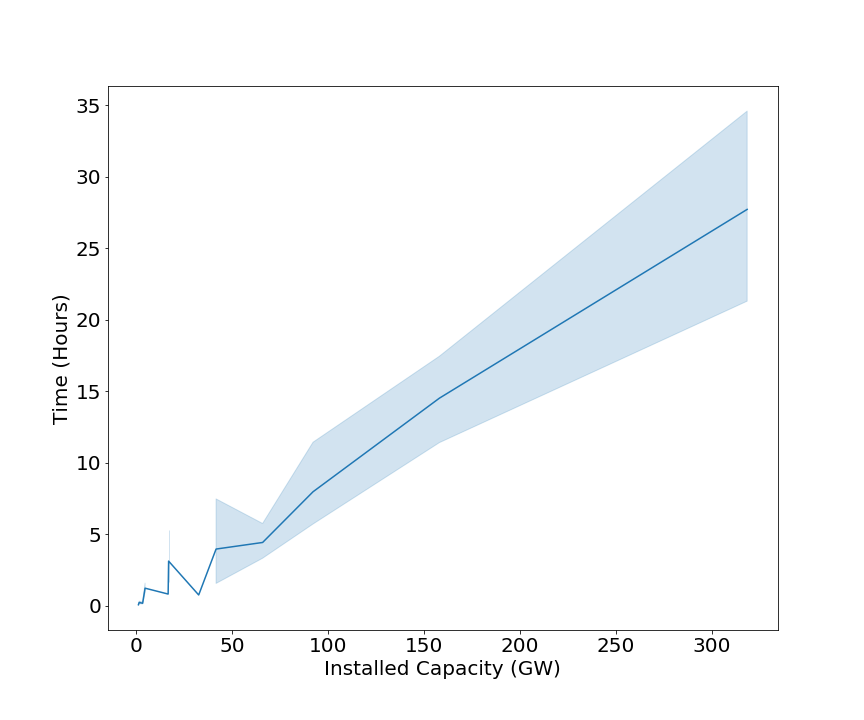
\includegraphics[width=1\linewidth]{figures/timing_plot}
	\caption{Run times of different sized countries.}
	\label{fig:timingplot}
\end{figure}

Figure \ref{fig:timingplot} shows the running time for ElecSIM with varying installed capacity. We run the simulation with varying carbon taxes between 0, 20, 40 and \textsterling70 per tonne of \ce{CO2}. We varied demand between 2000MW and 320,000MW to see the effect of different sized countries on running time. The makeup of the electricity mix was achieve through stratified sampling of the UK electricity mix. 

The results show a generally linear time complexity with an increase in installed capacity leading to an increase in run time.

%\begin{itemize}
%	\item Validation of model 
%	\begin{itemize}
%		\item Compare price duration curve
%		\item Compare power plant costs and NPV calculations
%		\item Look number of steps ahead to compare electricity mix and compare to actual (cross-validation)
%	\end{itemize} 
%	\item Performance metrics - Comparison with EMLab, PowerACE (15 minute run time)
%	\begin{itemize}
%		\item Memory, disk size, runtime
%		\item Increase in time complexity with additional data.
%	\end{itemize}
%\end{itemize}
